\chapter{Introduction}
\label{ch:intro}

\section{Motivation}
\label{sec:motivation}

Debugging is a task that every developer and software engineer will have to go
through while writing code. It's often a
tedious process that involves manually checking the code and running it multiple
times to simply find the location of the error in the code. Finding possible
solutions to fix the fault would then be the next step in the debugging process.
In Postman's 2020 State of the API Report, developers reported allocating
seventeen percent of their time debugging and manually testing their code.
Fig \ref{fig:development_time} demonstrates that debugging makes up the
second most time consuming task for API developers.
In an effort to facilitate and automate this process, different tools have been
created to guide the developer in locating error(s) and suggesting how to go
about fixing them. Solving this problem can significantly increase the
efficiency of experienced developers and increase the quality of the code they
ship. Additionally, a solution can help in decreasing the time spent on
debugging and allow developers to focus on other important tasks.
Beginner and novice developers can also benefit greatly from tools
that facilitate the debugging process, which could ease the learning process and help
them avoid making mistakes. Overall, contributions to this field of study could
assist developers and software engineer of all levels.
With special concentration on novice and beginner developers in an educational
environment, this research implements and evaluates a tool focused on helping
developers find bugs in their code.

% TODO: create citation
\begin{figure}[!htb]
	\begin{center}
		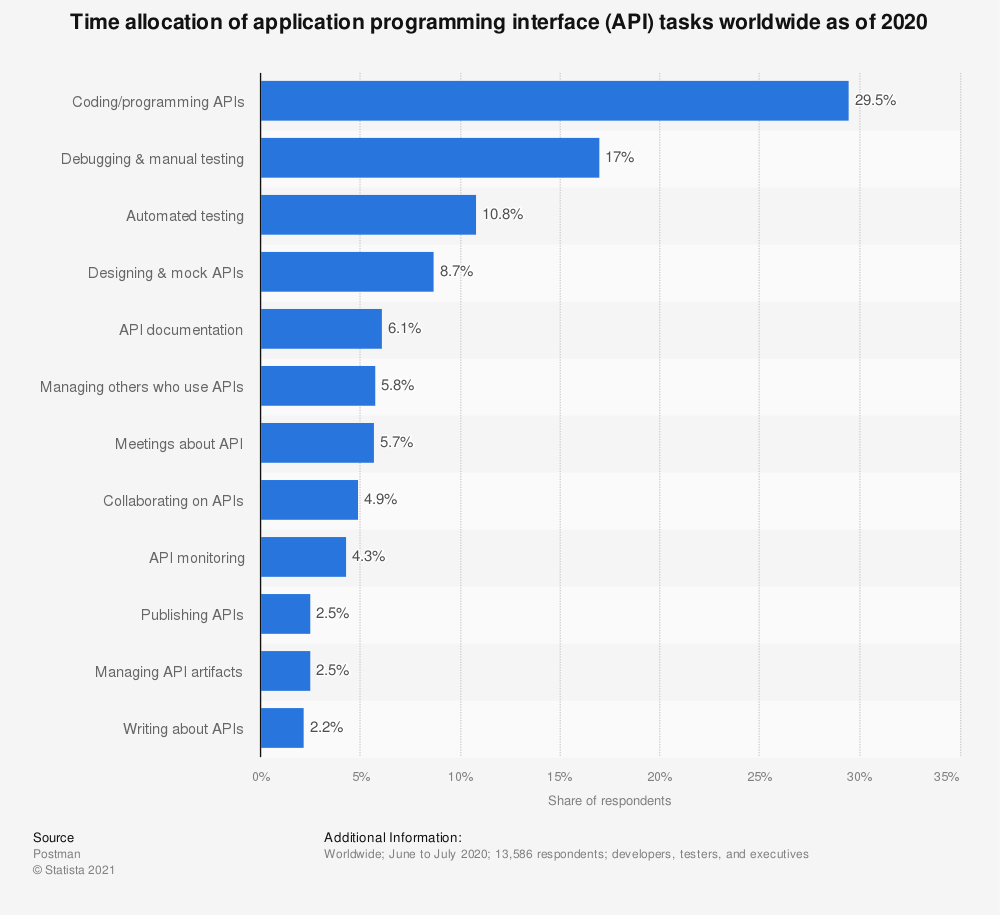
\includegraphics[width=\textwidth]{dev_time_stat.png}
		\caption{\label{fig:development_time} API Developers Time Allocation}
	\end{center}
\end{figure}

\section{Background}
\label{sec:background}

\subsection{Debugging and Fault Localization}
\label{subsec:DebuggingAndAFL}

The debugging process for developers typically starts when a ``bug'',
unexpected/incorrect behavior has been observed. One of many ways to check
whether incorrect behavior is taking place is through unit testing. This type of
testing consists of a set of test cases that check the different functionalities of the
code by asserting that expected output and actual output match. When a test case
fails due to a mismatch in the assertion, the search for the causing bug begins.
This research focuses on this crucial step in debugging and aims to guide the
search process by setting priority locations for the developers to search in.

Debugger tools have often been used to find and fix bugs in code, and while they
have several benefits, they also have drawbacks. Debuggers provide the developer
with a way to essentially pause the runtime of a program using breakpoints to display
information about the state of different variables and function call stack.
Through debuggers, developers can run the code line by line until an unexpected
behavior is detected. There is no denial that debuggers are very effective,
however, using them can be time consuming, especially for complex bugs.
Additionally, debuggers require that the code is ran during the debugging
process which could increase the time needed to debug and might not always be
feasible. With these drawbacks in mind, several automated fault localization (AFL)
algorithms and approaches have been studied to increase the
efficiency of the debugging process.

% TODO: find the sources that explores different types of AFL
Automated Fault Localization approaches perform different types of analysis to
the code and attempt to find the location of existing faults. Some approaches
use trained artificial intelligence models to assess the code and make
predictions on where some faults may exist. Others construct and analyse
abstract syntax trees to look for potential errors. On the other hand,
approaches such as spectrum-based fault localization rely on data collected
during the runtime of the code to ``identify the part of the program whose
activity correlates most with the detection of errors'' \cite{ABREU20091780}.
More specifically, the results of the program's test suite is used to find this
correlation. This latter approach is the focus of this research, where a
spectrum-based automated fault localization tool is implemented.

\subsection{Spectrum Based Fault Localization}
\label{subsec:SpectrumBased}

The reliance of spectrum based fault localization (SFL) on data already
collected during running and testing reduces the overall cost of debugging since
there is no need to rerun the code. When focusing on collected test suite data,
SFL becomes even more applicable since it can be integrated with many unit test
frameworks. In addition to the per-test outcome of a test suite, per-test
coverage data is also used in SFL to identify which lines are executed by each
test case. Once this data is collected following a test suite run, SFL assesses
the suspiciousness of code blocks depending on how many failing test cases run
those blocks. From a logical point of view, the block/line of code executed the
most by a failing test case is the most likely to contain the fault. SFL also
uses various equations to calculate and quantitatively evaluate the
suspiciousness all blocks of code.

While SFL can provide great insight for developers looking to debug their code,
it's not always reliable or applicable. In the case where a test suite hasn't
been fully implemented, the output of SFL may not narrow down potentially faulty
code to a single line. Additionally, ties in suspiciousness scores between lines
and blocks may come up, which may not offer the developer any valuable output.
Overall limitations of SFL will be discussed and acknowledged
in evaluating the outcome of this research.

% TODO: include other criticism of SFL

\section{Main Aims}
\label{sec:aims}

With the demonstrated importance of debugging tools and strategies that increase
developer efficiency, this research implements and evaluates an AFL tool to
assist in debugging code. AFLuent is built using  Python programming
language and uses SFL approach to identify faults in a
program. Stack Overflow 2021 Developer Survey identified Python as the third
most used programming/markup language used by developers worldwide. With that in
mind, an automated fault localization tool in Python can reach a wide audience
in various fields such as data science and AI who may have various levels of
experience. By implementing AFLuent using Python, powerful libraries and
packages such as Pytest and Coverage.py can be used to collect test suite data
in order to calculate suspiciousness.

Following the implementation of AFLuent, this research evaluates the
tool's performance and accuracy. Several open source projects
available on GitHub are handpicked to run AFLuent against. A representative
sample of projects with various sizes and relevance will be used to collect
data. Mutation testing libraries are used to introduce bugs into the code,
following that step, AFLuent uses the resulting test suite data to identify the
introduced fault. Through this process, AFLuent's performance and ability to
correctly identify and rank suspicious statements/and blocks is assessed.

\section{Research Question}
\label{sec:researchq}

% TODO: edit this to fit in
With the importance of fault localization algorithms in mind, and the need for a
functional and robust tool for beginners, this research proposal
seeks to answer the following general research questions:

\begin{center}
	\emph{RQ1. What are the best available techniques to automate the process of
	fault localization using test coverage data?
	}
\end{center}

This question is focused on the theoretical and evaluative purpose of this
proposed work. However, it's very helpful in building a foundational
understanding of automated fault localization, and assessing the results of the
research. Since this research question is general, it's further split into
smaller sub-questions discussed below.

\begin{center}
	\emph{RQ1.1. What are the most popular formulas for code suspiciousness
	created and evaluated by past literature?
	}
\end{center}

To answer this question, an extensive literature review is needed to understand
existing research on these formulas. Additionally, many studies contain
empirical evaluation of their formula/approach that distinguishes it from
others. All of these aspects will need to be taken into consideration when
deciding which formulas to implement and evaluate as part of the automated fault
localization tool.

\begin{center}
	\emph{RQ1.2. How should each selected formula/technique be empirically
	evaluated to reflect the accuracy of the resulting rankings?
	}
\end{center}

To ensure correctness and effectiveness, this research question requires that a
thorough process is planned for collecting data and testing the tool post
implementation. A more extensive discussion for this question will be addressed
in the evaluation section, which will outline the process of collecting data,
and conducting analysis on the results.

\begin{center}
	\emph{RQ2. How can automated fault localization techniques be implemented in
	Python as a novice developer friendly tool?
	}
\end{center}

This research question focuses on the implementation section
of this research where the result is a functional tool that can be used by
developers. Since the target audience of the proposed tool is novice developers,
special consideration is needed in regards to ease of use and installation.
The method of approach section will further expand on the planned steps to
answer this question.

\section{Thesis Outline}
\label{sec:outline}